\section{Transfer of 3D cloth model to the target Human and Virtual Try-On }  \label{section:clothtransfer}


\subsection{Transfer of 3D cloth model to the target Human} 

The 3D model and texture information obtained above are for the standard shape and posed person. To apply this information to the target human image, we have to apply the shape and pose parameters of estimated from SMPLify\cite{Bogo2016SMPLify} step.  In stead of apply the shape and pose parameters to the obtained clothed 3D model, we transferred the displacement of cloth vertices to the target human body model, because the application of new parameters to the Body model provide much natural results.      

Multiple option can be considered for the transferring. We could transfer the physical size of cloth or keep the fit, i.e., keep the displacement from the body to cloth vertex as before.  We simply decide the Fit-preserving option for showing more natural results for final fitting.  

Technically the displacement should be calculated locally. First we calculated the local coordinate at each vertices. We defines the local coordinates: surface normal vector as z -axis, and the vector to smallest indexed edge as x-axis, and their cross product vector as y-axis as the following equations.
 

\begin{align}
 u_{z} =  normal(V_{body})  \\
 u_{x} = u^{''}_{x}/ |u^{''}_{x} |, 
 u^{''}_{x} = u^{'}_{x} - u^{'}_{x} \cdot u_{z}, 
 u^{'}_{x} = (V_{argmin(N_V) } - V_{body}) \\
 u_{y}  =  u_z \otimes u_x,
\end{align} 
 where $N_V$ is the neighbor vertex of $V$.
 

The displacement is expressed in the local coordinates and then used the same way in the new target body surfaces for location transfer

\begin{equation}
\overrightarrow{d} = (d_x, d_y, d_z) = V_{clothed} - V_{body} \: in \: (u_x, u_y, u_z | V_{body})
\end{equation}


\begin{equation}
 V'_{clothed} = V'_{body} + \overrightarrow{d} \: in \: (u_x, u_y, u_z | V'_{body})
\end{equation}



\subsection{Blending of warped cloth with target human image}


This part is under implementation.

We first tried to use TOM. But we found when the reconstruction is not perfect the blending is not natural 

Other option is first reconstruct all the clothed information from the target user and overlay the transferred cloth.


\begin{figure}
\centering
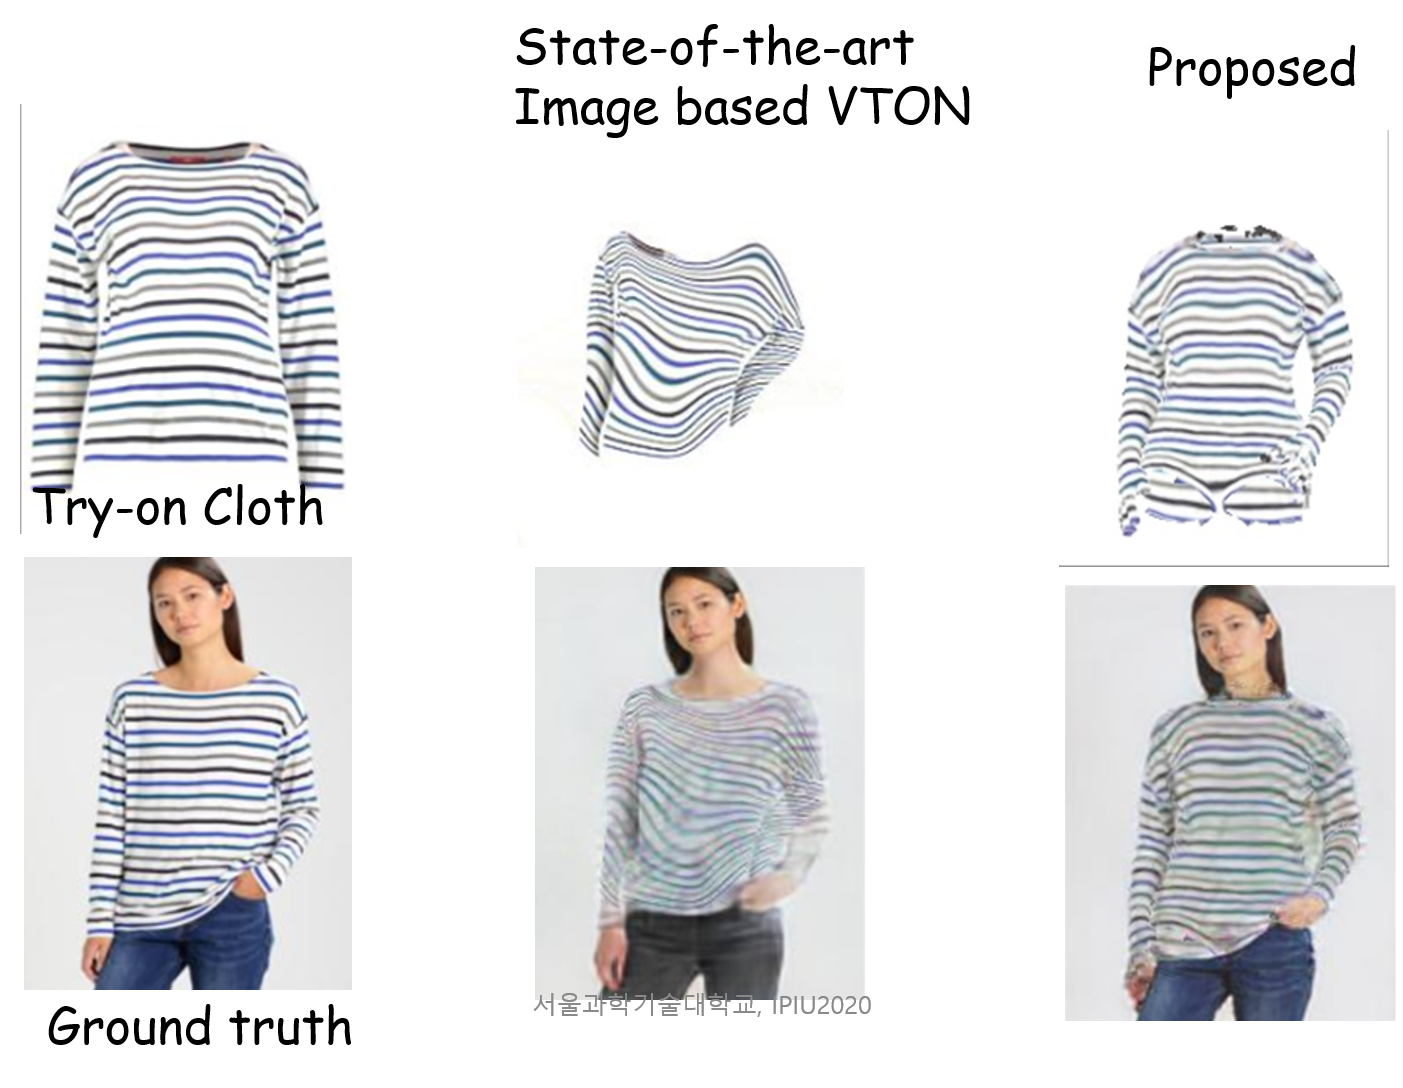
\includegraphics[height=6.5cm, scale=1]{figures/vton_result1.png} 
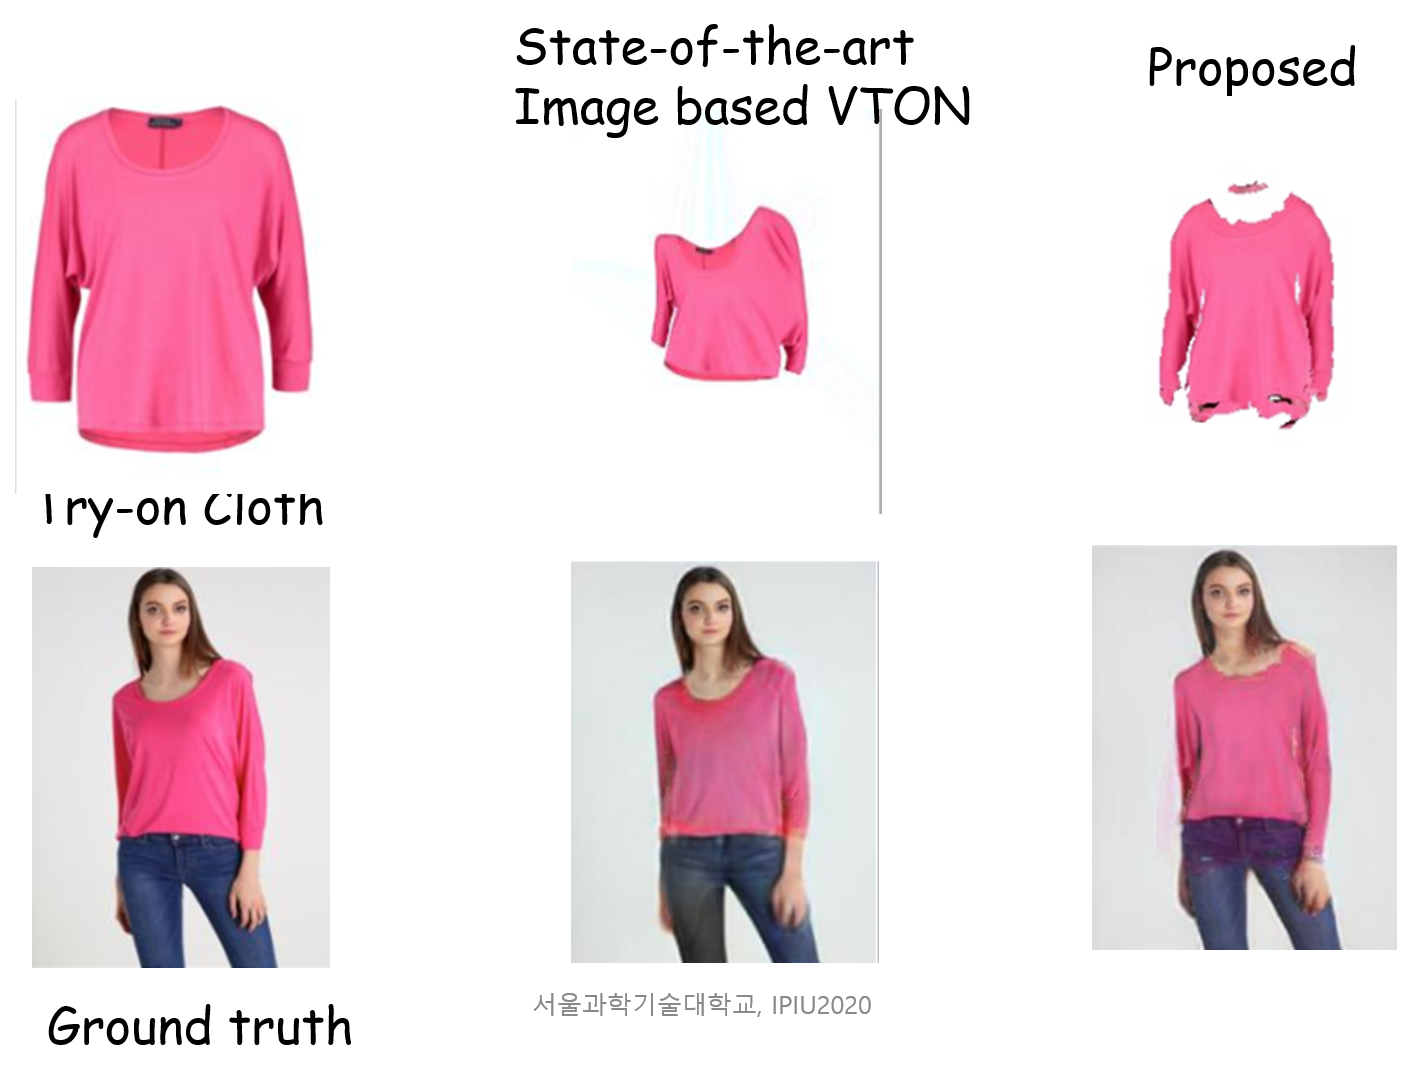
\includegraphics[height=6.5cm, scale=1]{figures/vton_result2.png} 
\caption{VTON results}
\label{fig:vtonresults}
\end{figure}




